\documentclass[colorlinks]{beamer}
  % compress
  %\documentclass[handout,xcolot=pdftex,dvipsnames,table]{beamer}
%\definecolor{mybg}{RGB}{255,255,204}
\definecolor{mybg}{RGB}{238,255,170}
\usepackage{minted}
\usepackage{graphicx}
\usepackage[english]{babel}
\usepackage{color}
\usepackage[utf8x]{inputenc}
%\usepackage{amsmath}
%\usepackage{beamerthemesplit}
%\usemintedstyle{trac}

\mode<presentation>
\setbeamercovered{invisible}
\usetheme{Warsaw}
\usecolortheme{dolphin}

\usefonttheme{serif}


\begin{document}
\setcounter{tocdepth}{2}

% Delete this, if you do not want the table of contents to pop up at
% the beginning of each subsection:
\AtBeginSection[]
{
  \begin{frame}<beamer>{Outline}
    \tableofcontents[currentsection]
  \end{frame}
}
\title{ Python in a Nutshell}
\subtitle
 {Part I: Python, ipython, language and OOP } % (optional)

\author[Velasco and Perera]{Manel Velasco,\inst{1} PhD and Alexandre Perera,\inst{1}$^{,}$\inst{2} PhD}

\institute[UPC] % (optional, but mostly needed)
{
  \inst{1}%
  Departament d'Enginyeria de Sistemes, Automatica i Informatica Industrial (ESAII)  \\
  Universitat Politecnica de Catalunya 
  \and 
  \inst{2}%
   Centro de Investigacion Biomedica en Red en Bioingenieria, Biomateriales y Nanomedicina (CIBER-BBN)  \\
    \href{mailto:Alexandre.Perera@upc.edu}{Alexandre.Perera@upc.edu}~\href{mailto:manel.velasco@upc.edu}{Manel.Velasco@upc.edu}
}
 

\date[Feb, 2013, Learning Python]{Introduction to Python for Engineering and Statistics\\
Febraury, 2013}

 %

%----------------------------FRAME------------------------------------
\begin{frame}[plain]
   %  \titlepage
   \maketitle
\end{frame}
%----------------------------FRAME------------------------------------
\begin{frame}[allowframebreaks]{Contents}
  \tableofcontents
  % You might wish to add the option [pausesections]
 \note[options]{aixo son notes}
\end{frame}
%-------------------------------------------------------------------
%---------------------------SECTION---------------------------------
%-------------------------------------------------------------------
\section{Introduction}



\subsection{Why Learn Python}
%----------------------------FRAME------------------------------------

\begin{frame}\frametitle{The scientist’s needs}
\small
\begin{itemize}
    \item Get data (simulation, experiment control)
    \item Manipulate and process data.
    \item Visualize results... to understand what we are doing!
    \item Communicate results: produce figures for reports or publications, write presentations.
\end{itemize}
\end{frame}

%----------------------------FRAME------------------------------------
\begin{frame}[fragile]\frametitle{Specifications}
\small
  \begin{itemize}
    \item We don’t want to re-program the plotting of a curve, a Fourier transform or a fitting algorithm. Don’t reinvent the wheel! We need building blocks 
    \item Easy to learn: computer science is neither our job nor our education
    \item The code should be as readable as a book
    \item Efficient code that executes quickly... but needless to say that a very fast code becomes useless if we spend too much time writing it. So, we need both a quick development time and a quick execution time
    \item A single environment/language for everything
\end{itemize}

\end{frame}

%----------------------------FRAME------------------------------------
\begin{frame}\frametitle{ Existing solutions I}
\begin{itemize}
    \item Compiled languages: C, C++, Fortran, etc.
        \begin{itemize}
            \item Advantages:
                \begin{itemize}
                    \item \tiny Very fast. Very optimized compilers. For heavy computations, it’s difficult to outperform these languages.
                    \item \tiny Some very optimized scientific libraries have been written for these languages. Example: BLAS (vector/matrix operations)
                \end{itemize}
            \item Drawbacks:
                \begin{itemize}
                    \item \tiny Painful usage: no interactivity during development, mandatory compilation steps, verbose syntax (*, **, ::, \} , ; etc.), manual memory management (tricky in C). These are \textbf{difficult languages} for non computer scientists.
                 \end{itemize}
        \end{itemize}
 \end{itemize}

\end{frame}
\begin{frame}\frametitle{ Existing solutions II}
\begin{itemize}
    \item Scripting languages: Matlab   
        \begin{itemize}
            \item Advantages:
                \begin{itemize}
                    \item \tiny Very rich collection of libraries with numerous algorithms, for many different domains. Fast execution because these libraries are often written in a compiled language.
                    \item \tiny Pleasant development environment: comprehensive and well organized help, integrated editor, etc.
                    \item \tiny Commercial support is available. 
                \end{itemize}
            \item Drawbacks:
                \begin{itemize}
                    \item \tiny Base language is quite poor and can become restrictive for advanced users.
                    \item \textbf{Not free }
                \end{itemize}
        \end{itemize}
    \end{itemize}
\end{frame}

\begin{frame}\frametitle{ Existing solutions III}
 \begin{itemize}
    \item Other scripting languages: Scilab, Octave, Igor, R, IDL, etc.
        \begin{itemize}
            \item Advantages:
                \begin{itemize}
                     \item \tiny Open-source, free, or at least cheaper than Matlab.
                    \item \tiny Some features can be very advanced (statistics in R, figures in Igor, etc.)\end{itemize}
            \item Drawbacks:
                \begin{itemize}
                    \item \tiny Fewer available algorithms than in Matlab, and the language is not more advanced.
                    \item \tiny Some software are dedicated to one domain. Ex: Gnuplot or xmgrace to draw curves. These programs are very powerful, but they are restricted to a single type of usage, such as plotting.
                \end{itemize}
        \end{itemize}
\end{itemize}
\end{frame}

%----------------------------FRAME------------------------------------
\begin{frame}[fragile]\frametitle{Why not?}

 \begin{itemize}
    \item What about Python?
        \begin{itemize}
            \item Advantages:
                \begin{itemize}
                     \item \tiny Very rich scientific computing libraries (a bit less than Matlab, though)
                    \item \tiny Well thought out language, allowing to write very readable and well structured code: we “code what we think”.
                    \item \tiny Many libraries for other tasks than scientific computing (web server management, serial port access, etc.)
                    \item \tiny Free and open-source software, widely spread, with a vibrant community.
                \end{itemize}
            \item Drawbacks:
                \begin{itemize}
                    \item \tiny Less pleasant development environment than, for example, Matlab. (More geek-oriented).
                    \item \tiny Not all the algorithms that can be found in more specialized software or toolboxes. 
                \end{itemize}
        \end{itemize}
\end{itemize}
\begin{block}{\begin{center}
    It is not a must
\end{center}}
\begin{center}
You don't need to use Python... but  what the hell,\\ \textbf{why not?}\end{center}
\end{block}


\end{frame}

\subsection{Python History}

%----------------------------FRAME------------------------------------
\begin{frame}[fragile]\frametitle{History}
\begin{columns}[T]
    \begin{column}{.7\textwidth}
        \begin{block}{\centering History}
\small
            \begin{itemize}
                 \item Python 1.0 - January 1994
                    \begin{itemize}
\tiny
                        \item Python 1.5 - December 31, 1997
                        \item Python 1.6 - September 5, 2000
                    \end{itemize}
                \item Python 2.0 - October 16, 2000
                    \begin{itemize}
\tiny
                        \item Python 2.1 - April 17, 2001
                        \item Python 2.2 - December 21, 2001
                        \item Python 2.3 - July 29, 2003
                        \item Python 2.4 - November 30, 2004
                        \item Python 2.5 - September 19, 2006
                        \item Python 2.6 - October 1, 2008
                        \item \textbf{Python 2.7 - July 3, 2010}
                    \end{itemize}
                \item Python 3.0 - December 3, 2008
                    \begin{itemize}
\tiny
                        \item Python 3.1 - June 27, 2009
                        \item Python 3.2 - February 20, 2011
                        \item Python 3.3 - September 29, 2012
                    \end{itemize}
            \end{itemize}
        \end{block}
    \end{column}
    \begin{column}{.3\textwidth}
        \begin{block}{ \centering  Guido van Rossum}
            \begin{center}
                Conceived in the late 1980s by 
                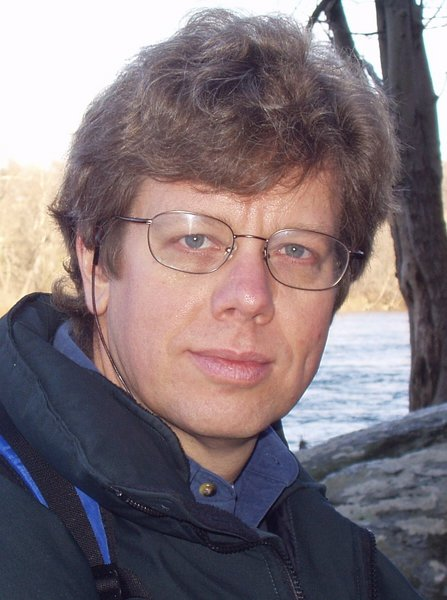
\includegraphics[scale=0.2]{figs/Guido_van_Rossum.jpg}
            \end{center}
        \end{block}
    \end{column}
  \end{columns}
\end{frame}


\subsection{Installing Python}

%----------------------------FRAME------------------------------------
\begin{frame}[fragile]\frametitle{Installation}

  \begin{columns}[T]
    \begin{column}{.4\textwidth}
        \begin{block}{\centering Linux}
\begin{center}
    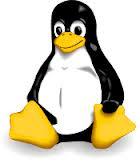
\includegraphics[scale=0.3]{figs/linux.jpg}
\end{center}
                  apt-get install python
        \end{block}
    \end{column}
    \begin{column}{.6\textwidth}
        \begin{block}{ \centering  Windows}
\centering

\begin{center}

\includegraphics[scale=0.3]{figs/windows.jpg}
\end{center}    
            Go to \textbf{http://www.python.org/getit/}
            and download 
\textbf{Python 2.7.3 Windows Installer}
        \end{block}        
    \end{column}
  \end{columns}
\end{frame}



\subsection{Python Resources}
%----------------------------FRAME------------------------------------
\begin{frame}[fragile]\frametitle{Resources}
\begin{block}{HELP!!!}
\textbf{http://python.org}
\begin{center}
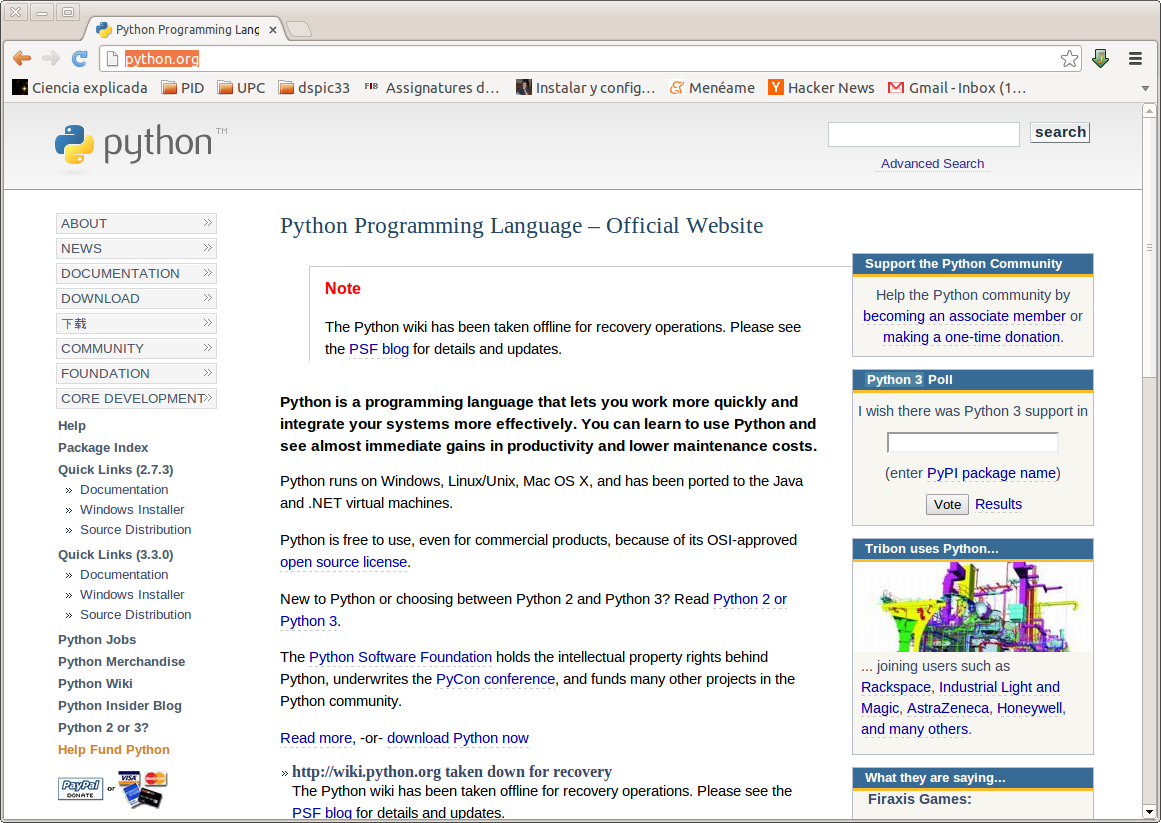
\includegraphics[scale=0.15]{figs/python__org.jpg}
\end{center}  
\end{block}
  
\end{frame}
%-------------------------------------------------------------------
%---------------------------SECTION---------------------------------
%-------------------------------------------------------------------

\section{Working with Python}

\subsection{Workflow}

%----------------------------FRAME------------------------------------
{
\usebackgroundtemplate{
  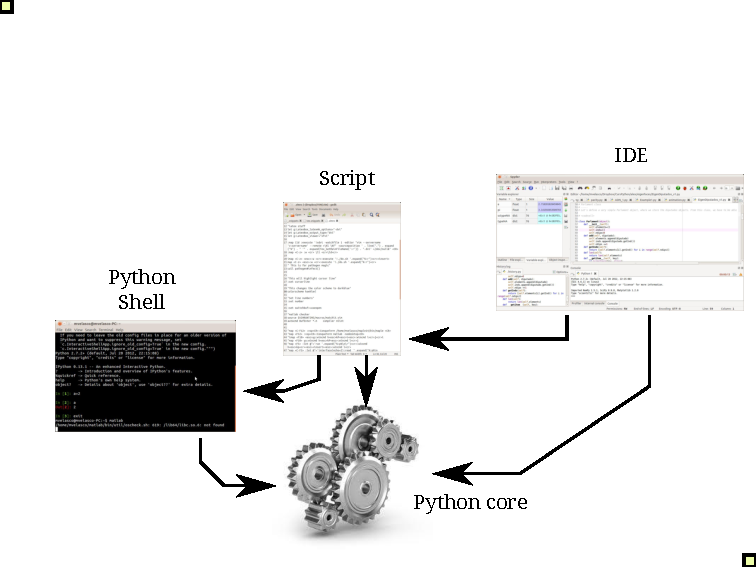
\includegraphics[width=\paperwidth,height=\paperheight]{figs/workflow.pdf}
}

\begin{frame}[fragile]\frametitle{Workflow}
\end{frame}
}
%----------------------------FRAME------------------------------------
\begin{frame}[fragile]\frametitle{Python core}
 
 \begin{columns}[T]
    \begin{column}{.7\textwidth}
        \begin{block}{\centering Python Core}
\small Python is open, is just an specification, thus there are many Python implementations:
\begin{description}
\scriptsize    
    \item[CPython] The default (C, C++)
    \item[CLPython] Lisp implementation of Python
    \item[Jython] The java implementation of Python
    \item[PyPy] The python implementation of Python
    \item [IronPython] C\# implementation
\end{description}
        \end{block}
    \end{column}
    \begin{column}{.3\textwidth}
\begin{center}
Python Core
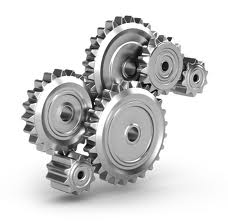
\includegraphics[scale=0.3]{figs/gears.jpg}
\end{center}    
    \end{column}
  \end{columns}
\end{frame}


\subsection{ipython vs. CLI}

%----------------------------FRAME------------------------------------
\begin{frame}[fragile]\frametitle{Python Shell}
        \begin{block}{\centering Python Shell}
\small There are many tools to drive directly with Python, the most remarkable are: 
    \begin{description}
\scriptsize    
        \item[CLIPython] The default one
        \item[IPython] Enhanced (VERY enhanced) default shell
    \end{description}
\end{block}
\begin{figure}
\begin{minipage}[b]{0.45\linewidth}
\centering
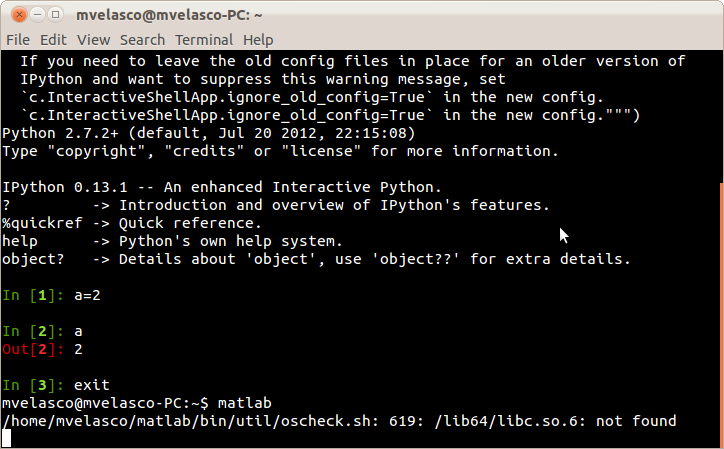
\includegraphics[width=\textwidth]{figs/commandline.jpg}
\end{minipage}
\hspace{0.5cm}
\begin{minipage}[b]{0.45\linewidth}
\centering
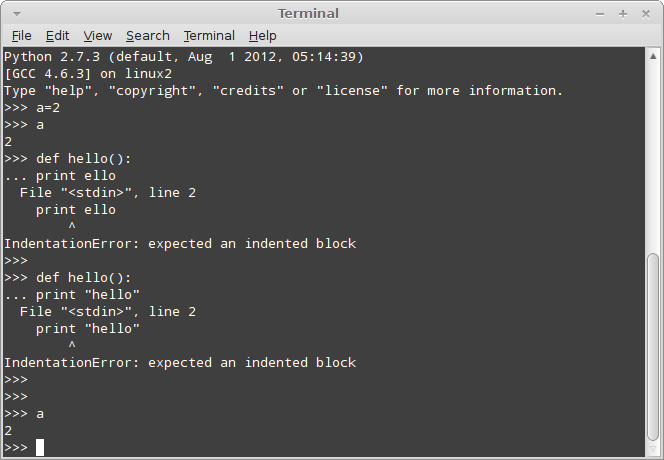
\includegraphics[width=\textwidth]{figs/commandline2.jpg}
\end{minipage}
\end{figure}    
\end{frame}




\subsection{Text Editors} % (fold)
%----------------------------FRAME------------------------------------
\begin{frame}[fragile]\frametitle{Text editors}
\begin{block}{Script editors}
 Any text editor is well suited for creating scripts with python, we recommend some features on it:
\begin{itemize}
    \item Tab substitution
    \item Code snippets
    \item Autocompletion
\end{itemize}
In the Linux wild, Vim and Emacs are both well suited.
\end{block}

\end{frame}

\subsection{IDEs}
%----------------------------FRAME------------------------------------
\begin{frame}[fragile]\frametitle{IDEs}
 \begin{block}{Most Valuable IDEs}
 \begin{description}
     \item[Spyder] The Matlab-like environment, scientist oriented.
    % \item [EDP] Enthought Python Distribution, complete set of tools.
Scientist oriented
     \item[Eclipse-PyDEV] Big project oriented  
 \end{description}
 \end{block}
\begin{center}
    \textbf{DEMO}
\end{center}

\end{frame}

\subsection{Notebook}
%----------------------------FRAME------------------------------------
\begin{frame}[fragile]\frametitle{Notebook}
\begin{block}{An HTML Notebook IPython}
The IPython Notebook consists of two related components:
\begin{itemize}
    \item An JSON based Notebook document format for recording and distributing Python code and rich text.
\item A \textbf{web-based user interface} for authoring and running notebook documents.
\end{itemize}
\end{block}
\begin{center}
    \textbf{DEMO}
\end{center}
\end{frame}

%-------------------------------------------------------------------
%---------------------------SECTION---------------------------------
%-------------------------------------------------------------------


\section{Getting Started With Python}

\subsection{Introduction}
%----------------------------FRAME------------------------------------
\begin{frame}[fragile]\frametitle{First step}
\begin{block}{\centering STEP 1}
\centering Start the interpreter and type in
\end{block}
  %-------------------------------CODE
\begin{minted}[bgcolor=mybg,frame=lines,mathescape]{python}
>>> print "Hello, world"
Hello, world
\end{minted}

\begin{block}{}
\centering Welcome to Python,\\ you just executed your first Python instruction, congratulations!
\end{block}
%-------------------------------END CODE
\end{frame}

%----------------------------FRAME------------------------------------
\begin{frame}[fragile]\frametitle{Second step}
\vspace{-0.1cm}
\begin{block}{\centering STEP 2}
\centering To get yourself started, type the following stack of instructions
\end{block}
 \begin{columns}[T]
\begin{column}{.5\textwidth}
%-------------------------------CODE
\tiny
\begin{minted}[bgcolor=mybg,frame=lines,mathescape]{python}
>>> a = 3
>>> b = 2*a
>>> type(b)
<type 'int'>
>>> print b
6
>>> a*b
18
>>> b = 'hello'
>>> type(b)
<type 'str'>
>>> b + b
'hellohello'
>>> 2*b
'hellohello'
\end{minted}

%-------------------------------END CODE

\end{column}
    \begin{column}{.5\textwidth}
\end{column}
\end{columns}
\end{frame}

%----------------------------FRAME------------------------------------
\begin{frame}[fragile]\frametitle{Second step}
\vspace{-0.1cm}
\begin{block}{\centering STEP 2}
\centering To get yourself started, type the following stack of instructions
\end{block}
 \begin{columns}[T]
\begin{column}{.5\textwidth}
%-------------------------------CODE
\tiny
\begin{minted}[bgcolor=mybg,frame=lines,mathescape]{python}
>>> a = 3
>>> b = 2*a
>>> type(b)
<type 'int'>
>>> print b
6
>>> a*b
18
>>> b = 'hello'
>>> type(b)
<type 'str'>
>>> b + b
'hellohello'
>>> 2*b
'hellohello'
\end{minted}

%-------------------------------END CODE

\end{column}
    \begin{column}{.5\textwidth}
    \begin{block}{\centering Observe that}
            \begin{itemize}
\scriptsize    
                \item We do not declare variables (hurrah!!!!!) 
                \item Variable type may be changed on the fly (hurrah!!!, hurrah!!!)
                \item There is a way to overload operators (hurrah!, hurrah!, hurrah!!!)\\
                \item There is a function that tell us the type of a variable.
            \end{itemize}
       \end{block}

\end{column}
\end{columns}
\end{frame}

\subsection{Basic Types}
%----------------------------FRAME------------------------------------
\begin{frame}[fragile]\frametitle{Types}
 \begin{columns}[T]
\begin{column}{.5\textwidth}
   \begin{block}{Integer}
 %-------------------------------CODE
\tiny
\begin{minted}[bgcolor=mybg,frame=lines,mathescape]{python}
>>> 1+1
2
>>> a=4
\end{minted}

 %-------------------------------END CODE
  \end{block}
 \begin{block}{Boolean}
%-------------------------------CODE
\tiny
\tiny
\begin{minted}[bgcolor=mybg,frame=lines,mathescape]{python}
>>> 3 > 4
False
>>> test = (3 > 4)
>>> test
False
>>> type(test)
<type 'bool'>
\end{minted}

%-------------------------------END CODE
\end{block}
\end{column}
    \begin{column}{.5\textwidth}
 \begin{block}{Float}
%-------------------------------CODE
\tiny
\begin{minted}[bgcolor=mybg,frame=lines,mathescape]{python}
>>> c=2.1
>>> 3.5/c
1.6666666666666665
\end{minted}


%-------------------------------END CODE
\end{block}
  \begin{block}{Complex}
%-------------------------------CODE
\tiny
\begin{minted}[bgcolor=mybg,frame=lines,mathescape]{python}
>>> a=1.5+0.5j
>>> a.real
1.5
>>> a.imag
0.5
>>> import cmath
>>> cmath.phase(a)
0.3217505543966422
\end{minted}

%-------------------------------END CODE  
  \end{block}

\end{column}
\end{columns}
\end{frame}
%----------------------------FRAME------------------------------------
\begin{frame}[fragile]\frametitle{Basic Calculator}
\begin{block}{A Python shell can therefore replace your pocket calculator, with the basic arithmetic operations +, -, *, /, \% (modulo) natively implemented:}
%-------------------------------CODE
\begin{minted}[bgcolor=mybg,frame=lines,mathescape]{python}
>>> 7 * 3.
21.0
>>> 2**10
1024
>>> 8 % 3
2
\end{minted}

%-------------------------------END CODE
\end{block}

\end{frame}
%----------------------------FRAME------------------------------------
\begin{frame}[fragile]\frametitle{WARNING!}
\begin{block}{Integer Division}
%-------------------------------CODE
\small
\begin{minted}[bgcolor=mybg,frame=lines,mathescape]{python}
>>> 3/2
1
\end{minted}

%-------------------------------END CODE
\end{block}
\begin{block}{Use floats}
%-------------------------------CODE
\tiny
\begin{minted}[bgcolor=mybg,frame=lines,mathescape]{python}
>>> 3 / 2.
1.5
>>> a = 3
>>> b = 2
>>> a / b
1
>>> a / float(b)
1.5
\end{minted}

%-------------------------------END CODE
\end{block}
\end{frame}
%----------------------------FRAME------------------------------------
\begin{frame}[fragile]\frametitle{Lists}
Python provides many efficient types of containers, in which collections of objects can be stored.
\begin{block}{Lists}
A list is an ordered collection of objects, that may have different types. For example
%-------------------------------CODE
\begin{minted}[bgcolor=mybg,frame=lines,mathescape]{python}
>>> l = [1, 2, 3, 4, 5]
>>> type(l)
<type 'list'>
\end{minted}

%-------------------------------END CODE
\end{block}
\end{frame}

%----------------------------FRAME------------------------------------
\begin{frame}[fragile]\frametitle{Lists}
\begin{block}{accessing individual objects contained in the list:}
%-------------------------------CODE
\tiny
\begin{minted}[bgcolor=mybg,frame=lines,mathescape]{python}
>>> l[2]
3
\end{minted}

%-------------------------------END CODE
\end{block}
\begin{block}{Counting from the end with negative indices:}
%-------------------------------CODE
\tiny
\begin{minted}[bgcolor=mybg,frame=lines,mathescape]{python}
>>> l[-1]
5
>>> l[-2]
4
\end{minted}

%-------------------------------END CODE
\end{block}
\begin{block}{{\color{green}\textbf{Warning Indexing starts at 0} }}
%-------------------------------CODE
\tiny
\begin{minted}[bgcolor=mybg,frame=lines,mathescape]{python}
>>> l[0]
1
\end{minted}

%-------------------------------END CODE
\end{block}
\end{frame}

%----------------------------FRAME------------------------------------
\begin{frame}[fragile]\frametitle{Lists}
\begin{block}{Slicing}
%-------------------------------CODE
\begin{minted}[bgcolor=mybg,frame=lines,mathescape]{python}
>>> l
[1, 2, 3, 4, 5]
>>> l[2:4]
[3, 4]
\end{minted}

%-------------------------------END CODE

\end{block}
\begin{block}{{\color{green}\textbf{Warning} }}
Warning Note that \textbf{l[start:stop]} contains the elements with indices i such as start $\le$ i $<$ stop (i ranging from start to stop-1). Therefore, \textbf{l[start:stop] has (stop-start) elements}.
\end{block}

\end{frame}

%----------------------------FRAME------------------------------------
\begin{frame}[fragile]\frametitle{Lists}
\begin{block}{}
Slicing syntax: l[start:stop:step]
\end{block}
\begin{block}{All slicing parameters are optional:}
%-------------------------------CODE
\begin{minted}[bgcolor=mybg,frame=lines,mathescape]{python}
>>> l
[1, 2, 3, 4, 5]
>>> l[3:]
[4, 5]
>>> l[:3]
[1, 2, 3]
>>> l[::2]
[1, 3, 5]
\end{minted}

%-------------------------------END CODE
\end{block}
\end{frame}

%----------------------------FRAME------------------------------------
\begin{frame}[fragile]\frametitle{Lists}
\begin{block}{The elements of a list may have different types:}
%-------------------------------CODE
\begin{minted}[bgcolor=mybg,frame=lines,mathescape]{python}
>>> l = [3, 2+3j, 'hello']
>>> l
[3, (2+3j), 'hello']
>>> l[1], l[2]
((2+3j), 'hello')
\end{minted}

%-------------------------------END CODE
\end{block}

\end{frame}
%----------------------------FRAME------------------------------------
\begin{frame}[fragile]\frametitle{Lists}
\vspace{-0.2cm}
\small
Python offers a large panel of functions to modify lists, or query them. Here are a few examples; for more details, see \href{http://docs.python.org/tutorial/datastructures.html#more-on-lists}{http://docs.python.org/tutorial/datastructures.html\#more-on-lists}
\vspace{-0.2cm}
\begin{block}{Add and remove elements}
\tiny
%-------------------------------CODE
\begin{minted}[bgcolor=mybg,frame=lines,mathescape]{python}
>>> l = [1, 2, 3, 4, 5]
>>> l.append(6)
>>> l
[1, 2, 3, 4, 5, 6]
>>> l.pop()
6
>>> l
[1, 2, 3, 4, 5]
>>> l.extend([6, 7]) # extend l, in-place
>>> l
[1, 2, 3, 4, 5, 6, 7]
>>> l = l[:-2]
>>> l
[1, 2, 3, 4, 5]
\end{minted}

%-------------------------------END CODE
\end{block}
\end{frame}
%----------------------------FRAME------------------------------------
\begin{frame}[fragile]\frametitle{Lists}
\vspace{-0.2cm}
\begin{block}{Reverse list}
%-------------------------------CODE
\tiny
\begin{minted}[bgcolor=mybg,frame=lines,mathescape]{python}
>>> r = l[::-1]
>>> r
[5, 4, 3, 2, 1]
\end{minted}

%-------------------------------END CODE
\end{block}
\vspace{-0.2cm}
\begin{block}{Concatenate and repeat}
%-------------------------------CODE
\tiny
\begin{minted}[bgcolor=mybg,frame=lines,mathescape]{python}
>>> r + l
[5, 4, 3, 2, 1, 1, 2, 3, 4, 5]
>>> 2 * r
[5, 4, 3, 2, 1, 5, 4, 3, 2, 1]
\end{minted}

%-------------------------------END CODE

\end{block}
\vspace{-0.2cm}
\begin{block}{Sort (in-place)}
%-------------------------------CODE
\tiny
\begin{minted}[bgcolor=mybg,frame=lines,mathescape]{python}
>>> r.sort()
>>> r
[1, 2, 3, 4, 5]
\end{minted}

%-------------------------------END CODE
\end{block}
\end{frame}
%----------------------------FRAME------------------------------------
\begin{frame}[fragile]\frametitle{Note}
\begin{block}{Methods and Object-Oriented Programming}
The notation r.method() (r.sort(), r.append(3), l.pop()) is our first example of object-oriented programming (OOP). Being a list, the object r owns the method function that is called using the notation '.'\\ No further knowledge of OOP than understanding the notation '.' is necessary for going through this tutorial.
\end{block}
\end{frame}
%----------------------------FRAME------------------------------------
\begin{frame}[fragile]\frametitle{Note}
\begin{block}{Discovering methods in ipython\\ tab-completion (press tab)}

\begin{minted} [bgcolor=mybg,frame=lines,bgcolor=mybg,frame=lines,bgcolor=mybg,frame=lines,mathescape]{python}
In [1]: r.
r.append   r.extend   r.insert   r.remove   r.sort     
r.count    r.index    r.pop      r.reverse 
\end{minted}
\end{block}
\end{frame}

%----------------------------FRAME------------------------------------
\begin{frame}[fragile]\frametitle{Strings}
\begin{block}{}
%-------------------------------CODE
\small
\begin{minted}[bgcolor=mybg,frame=lines,mathescape]{python}
s = 'Hello, how are you?'
s = "Hi, what's up"
s = '''Hello,                
       how are you'''# tripling the quotes allows the 
s = """Hi,
       what's up?""" # the string to span more than one line
\end{minted}

%-------------------------------END CODE
\end{block}
\end{frame}
%----------------------------FRAME------------------------------------
\begin{frame}[fragile]\frametitle{Strings}
\begin{block}{Indexing strings}
%-------------------------------CODE
\begin{minted}[bgcolor=mybg,frame=lines,mathescape]{python}
>>> a = "hello"
>>> a[0]
'h'
>>> a[1]
'e'
>>> a[-1]
'o'
\end{minted}

%-------------------------------END CODE
\end{block}
\end{frame}
%----------------------------FRAME------------------------------------
\begin{frame}[fragile]\frametitle{Strings}
\begin{block}{Substitution}
%-------------------------------CODE
\tiny
\begin{minted}[bgcolor=mybg,frame=lines,mathescape]{python}
>>> 'An integer: %i; a float: %f; another string: %s' % (1, 0.1, 'string')
'An integer: 1; a float: 0.100000; another string: string'
>>> i = 102.1
>>> filename = 'processing_of_dataset_%03d.txt'%i
>>> filename
'processing_of_dataset_102.txt'
\end{minted}

%-------------------------------END CODE
\end{block}
\end{frame}

%----------------------------FRAME------------------------------------
\begin{frame}[fragile]\frametitle{Challenge}
  \begin{block}{5 seconds challenge}
  In ipython, create a list and check its methods with the tab-completion feature
  \end{block}
\end{frame}

%----------------------------FRAME------------------------------------
\begin{frame}[fragile]\frametitle{Strings}
\begin{block}{Slicing}
%-------------------------------CODE
\tiny
\begin{minted}[bgcolor=mybg,frame=lines,mathescape]{python}
>>> a = "hello, world!"
>>> a[3:6] # 3rd to 6th (excluded) elements: elements 3, 4, 5
'lo,'
>>> a[2:10:2] # Syntax: a[start:stop:step]
'lo o'
>>> a[::3] # every three characters, from beginning to end
'hl r!'
\end{minted}

%-------------------------------END CODE
\end{block}
BUT...
\end{frame}

%----------------------------FRAME------------------------------------
\begin{frame}[fragile]\frametitle{Strings}
\begin{block}{You can't change them in this way}
\tiny
\begin{minted} [bgcolor=mybg,frame=lines,bgcolor=mybg,frame=lines,bgcolor=mybg,frame=lines,mathescape]{python}
In [1]: a = "hello, world!"
In [2]: a[2] = 'z'
-----------------------------------------------------------
TypeError              Traceback (most recent call last)

/home/mvelasco/Curs_Python/<ipythonconsole> in <module>()

TypeError: 'str' object does not support item assignment

\end{minted}
\end{block}
    \centering
    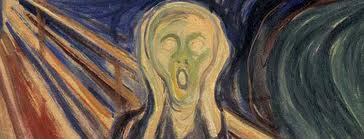
\includegraphics[scale=0.5]{figs/grito.jpg}
\end{frame}

\subsection{Mutable and immutable}
%----------------------------FRAME------------------------------------
\begin{frame}[fragile]\frametitle{PAY ATTENTION}
\begin{block}{}
\centering
\huge
{\color{red}\textbf{NEXT SET OF SLIDES ARE VERY IMPORTANT!!!}}
\end{block}
\end{frame}
%----------------------------FRAME 2 cols------------------------------
\begin{frame}[fragile]\frametitle{Mutable and immutable types}
\begin{columns}[c]
\column{0.5\textwidth}
\begin{block}{Immutable types}
\begin{itemize}
    \item integer
\item float
\item complex
\item boolean 
\item strings
\end{itemize}
\end{block}
\column{0.5\textwidth}
\begin{block}{Mutable}
\begin{itemize}
    \item Lists
\end{itemize}
\end{block}
\end{columns}
\end{frame}

%----------------------------FRAME 2 cols------------------------------
{
\usebackgroundtemplate{
  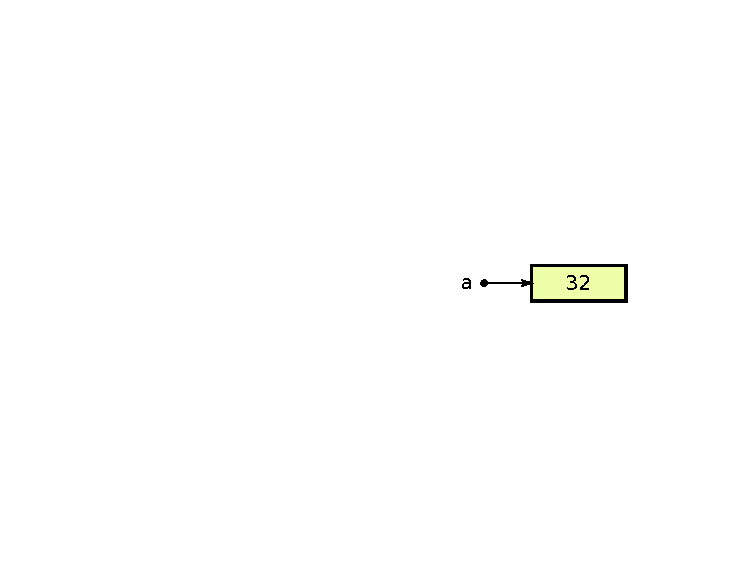
\includegraphics[width=\paperwidth,height=\paperheight]{figs/mutable1.pdf}
}

\begin{frame}[fragile]\frametitle{Immutable types}
\begin{columns}[c]
\column{0.5\textwidth}
\begin{block}{Create an immutable element}
%-------------------------------CODE
\begin{minted}[bgcolor=mybg,frame=lines,mathescape]{python}
>>> a=32
\end{minted}

%-------------------------------END CODE
\end{block}
\column{0.5\textwidth}
\end{columns}

\end{frame}
}

%----------------------------FRAME 2 cols------------------------------
{
\usebackgroundtemplate{
  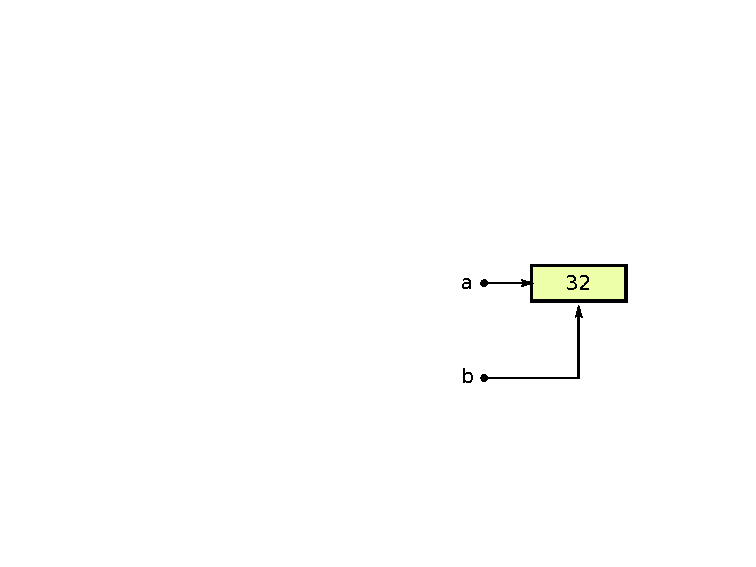
\includegraphics[width=\paperwidth,height=\paperheight]{figs/mutable2.pdf}
}

\begin{frame}[fragile]\frametitle{Immutable types}
\begin{columns}[T]
\column{0.5\textwidth}
\begin{block}{"copy" it}
%-------------------------------CODE
\begin{minted}[bgcolor=mybg,frame=lines,mathescape]{python}
>>> a=32
>>> b=a
\end{minted}

%-------------------------------END CODE
\end{block}
\column{0.5\textwidth}
\end{columns}

\end{frame}
}

%----------------------------FRAME 2 cols------------------------------
{
\usebackgroundtemplate{
  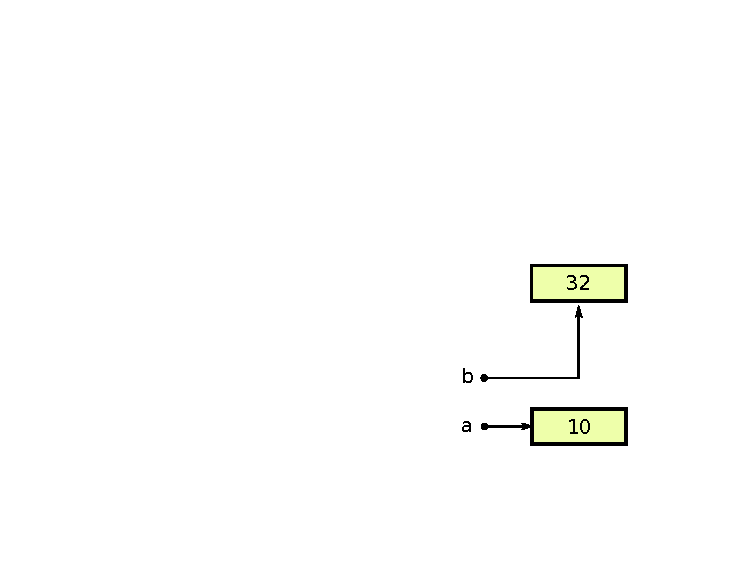
\includegraphics[width=\paperwidth,height=\paperheight]{figs/mutable3.pdf}
}

\begin{frame}[fragile]\frametitle{Immutable types}
\begin{columns}[T]
\column{0.5\textwidth}
\begin{block}{Change the original object}
%-------------------------------CODE
\begin{minted}[bgcolor=mybg,frame=lines,mathescape]{python}
>>> a=32
>>> b=a
>>> a=10
>>> b
32
\end{minted}

%-------------------------------END CODE
\end{block}
\column{0.5\textwidth}
\end{columns}

\end{frame}
}
%----------------------------FRAME 2 cols------------------------------
{
\usebackgroundtemplate{
  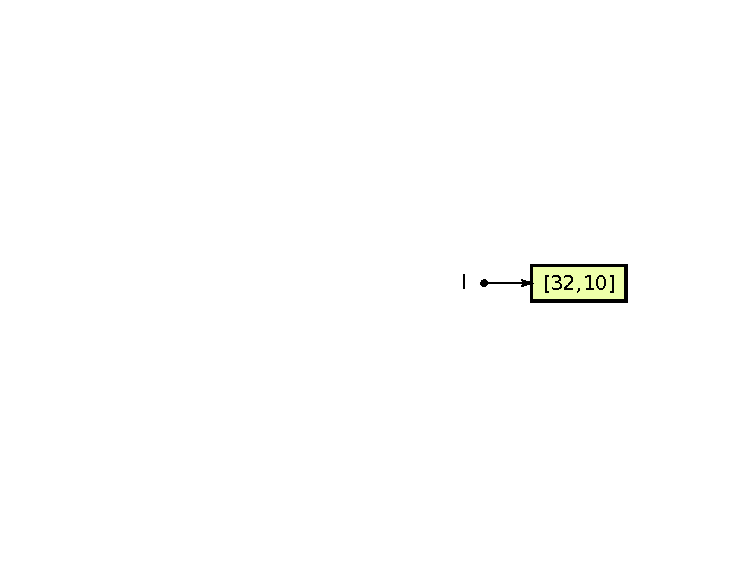
\includegraphics[width=\paperwidth,height=\paperheight]{figs/mutable4.pdf}
}

\begin{frame}[fragile]\frametitle{Mutable types}
\begin{columns}[T]
\column{0.5\textwidth}
\begin{block}{Create a mutable type}
%-------------------------------CODE
\begin{minted}[bgcolor=mybg,frame=lines,mathescape]{python}
>>> l=[32,10]
\end{minted}

%-------------------------------END CODE
\end{block}
\column{0.5\textwidth}
\end{columns}

\end{frame}
}

%----------------------------FRAME 2 cols------------------------------
{
\usebackgroundtemplate{
  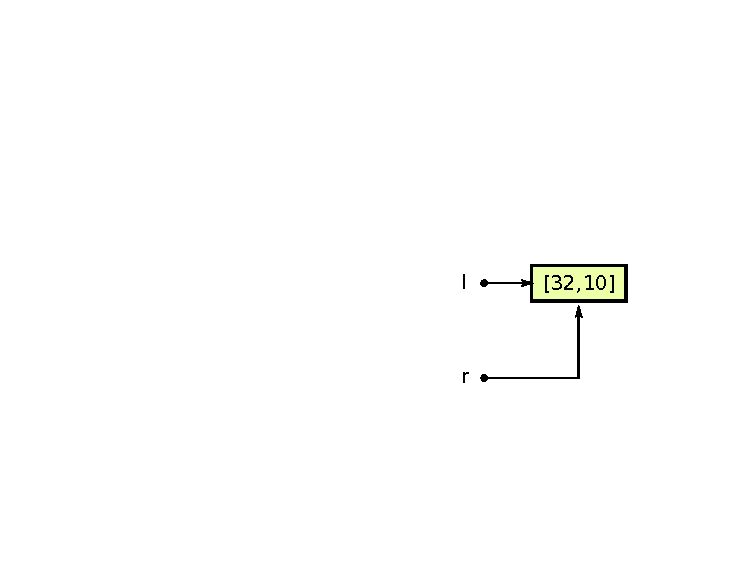
\includegraphics[width=\paperwidth,height=\paperheight]{figs/mutable5.pdf}
}

\begin{frame}[fragile]\frametitle{Mutable types}
\begin{columns}[T]
\column{0.5\textwidth}
\begin{block}{"Copy" it}
%-------------------------------CODE
\begin{minted}[bgcolor=mybg,frame=lines,mathescape]{python}
>>> l=[32,10]
>>> r=l
\end{minted}

%-------------------------------END CODE
\end{block}
\column{0.5\textwidth}
\end{columns}

\end{frame}
}

%----------------------------FRAME 2 cols------------------------------
{
\usebackgroundtemplate{
  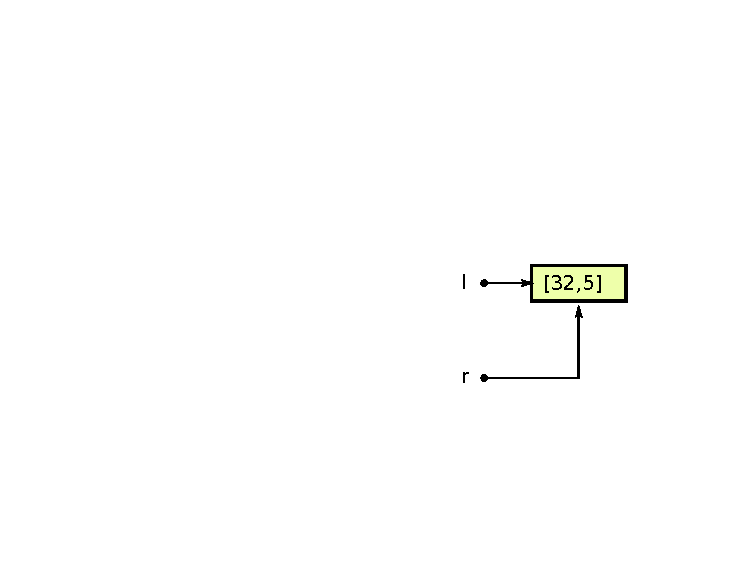
\includegraphics[width=\paperwidth,height=\paperheight]{figs/mutable6.pdf}
}

\begin{frame}[fragile]\frametitle{Mutable types}
\begin{columns}[T]
\column{0.5\textwidth}
\begin{block}{Change the original object}
%-------------------------------CODE
\begin{minted}[bgcolor=mybg,frame=lines,mathescape]{python}
>>> l=[32,10]
>>> r=l
>>> l[1]=3
>>> r
[32, 3]
\end{minted}

%-------------------------------END CODE
\end{block}
\column{0.5\textwidth}
\end{columns}

\end{frame}
}

%----------------------------FRAME------------------------------------
\begin{frame}[fragile]\frametitle{Challenge}
  \begin{block}{1 minute challenge}
  Create a list A, create a list B that contains A, copy the list B into C, modify A and check C value
  \end{block}
\end{frame}

%----------------------------FRAME 2 cols------------------------------

\begin{frame}[fragile]\frametitle{Visited Types}
\begin{columns}[T]
\column{0.5\textwidth}
\begin{block}{Already seen types}
\begin{itemize}
    \item boolean
\item integer
\item float
\item complex
\item string
\item list
\end{itemize}
\end{block}
\column{0.5\textwidth}
\begin{block}{Pending Types}
\begin{itemize}
    \item Dictionary
\item Tuple
\item Set
\end{itemize}
\end{block}
\end{columns}

\end{frame}


%----------------------------FRAME------------------------------------
\begin{frame}[fragile]\frametitle{Dictionary}
  \begin{block}{A dictionary is basically an efficient table that maps keys to values. It is an unordered container:}
  %-------------------------------CODE
\tiny
\begin{minted}[bgcolor=mybg,frame=lines,mathescape]{python}
>>> tel = {'emmanuelle': 5752, 'sebastian': 5578}
>>> tel['francis'] = 5915
>>> tel
{'sebastian': 5578, 'francis': 5915, 'emmanuelle': 5752}
>>> tel['sebastian']
5578
>>> tel.keys()
['sebastian', 'francis', 'emmanuelle']
>>> tel.values()
[5578, 5915, 5752]
>>> 'francis' in tel
True
\end{minted}

  %-------------------------------END CODE
  \end{block}
\end{frame}

%----------------------------FRAME------------------------------------
\begin{frame}[fragile]\frametitle{Dictionary}
\begin{block}{A dictionary can have keys (resp. values) with different types:}
%-------------------------------CODE
\begin{minted}[bgcolor=mybg,frame=lines,mathescape]{python}
>>> d = {'a':1, 'b':2, 3:'hello'}
>>> d
{'a': 1, 3: 'hello', 'b': 2}
\end{minted}

%-------------------------------END CODE
\end{block}
\end{frame}

%----------------------------FRAME------------------------------------
\begin{frame}[fragile]\frametitle{Challenge}
\begin{block}{1 minute challenge}
Are Dicts mutable?
\end{block}
\end{frame}

%----------------------------FRAME------------------------------------
\begin{frame}[fragile]\frametitle{Tuples}
\begin{block}{The elements of a tuple are written between parentheses, or just separated by commas:}
%-------------------------------CODE
\begin{minted}[bgcolor=mybg,frame=lines,mathescape]{python}
>>> t = 12345, 54321, 'hello!'
>>> t[0]
12345
>>> t
(12345, 54321, 'hello!')
>>> u = (0, 2)
\end{minted}

%-------------------------------END CODE
\end{block}
\end{frame}

%----------------------------FRAME------------------------------------
\begin{frame}[fragile]\frametitle{Sets}
\begin{block}{unordered, unique items:}
 %-------------------------------CODE
\begin{minted}[bgcolor=mybg,frame=lines,mathescape]{python}
>>> s = set(('a', 'b', 'c', 'a'))
>>> s
set(['a', 'c', 'b'])
>>> s.difference(('a', 'b'))
set(['c'])
\end{minted}

 %-------------------------------END CODE
\end{block}
\end{frame}

%----------------------------FRAME------------------------------------
\begin{frame}[fragile]\frametitle{Challenge}
  \begin{block}{2 minutes challenge}
\begin{itemize}
    \item Are tuples mutable?
\item Which are the methods of tuples?
\item Are Sets mutable?
\item Which are de methods of sets?
\end{itemize}
  
  \end{block}
\end{frame}


%----------------------------FRAME------------------------------------
\begin{frame}[fragile]\frametitle{Before going on...}
\begin{block}{Built-in functions}
\tiny
\begin{verbatim}
abs()	        divmod()	   input()	     open()	    staticmethod()
all()	        enumerate()	int()	       ord()	     str()
any()	        eval()	     isinstance()	pow()	     sum()
basestring()	 execfile()	 issubclass()	print()	   super()
bin()	        file()	     iter()	      property()	tuple()
bool()	       filter()	   len()	       range()	   type()
bytearray()	  float()	    list()	      raw_input()unichr()
callable()	   format()	   locals()	    reduce()	  unicode()
chr()	        frozenset()	long()	      reload()	  vars()
classmethod()	getattr()	  map()	       repr()	    xrange()
cmp()	        globals()	  max()	       reversed() zip()
compile()	    hasattr()	  memoryview() round()	   __import__()
complex()	    hash()	     min()	       set()	     apply()
delattr()	    help()	     next()	      setattr()	 buffer()
dict()	       hex()	      object()	    slice()	   coerce()
dir()	        id()	       oct()	       sorted()	  intern()
\end{verbatim}

\end{block}

\end{frame}


\subsection{Controlling execution flow}
%----------------------------FRAME------------------------------------
\begin{frame}[fragile]\frametitle{if/then/else}
\begin{block}{If}
\tiny
%-------------------------------CODE
\begin{minted}[bgcolor=mybg,frame=lines,mathescape]{python}
>>> if 2**2 == 4:
...     print 'Obvious!'
... 
Obvious!
\end{minted}

%-------------------------------END CODE

\end{block}
\begin{block}{Blocks are delimited by indentation}
\tiny
%-------------------------------CODE
\begin{minted}[bgcolor=mybg,frame=lines,mathescape]{python}
a = 10
if a == 1:
    print(1)
elif a == 2:
    print(2)
else:
    print('A lot')

\end{minted}
\begin{minted}[bgcolor=mybg,frame=lines,mathescape]{python}
A lot
\end{minted}

%-------------------------------END CODE
\end{block}
\end{frame}
%----------------------------FRAME 2 cols------------------------------
\begin{frame}[fragile]\frametitle{Conditional Expressions¶}
\begin{columns}[c]
\column{0.5\textwidth}
\tiny
\begin{block}{if object:}
Evaluates to False:
\begin{itemize}
    \item any number equal to zero (0, 0.0, 0+0j)
\item an empty container (list, tuple, set, dictionary, ...)
\item False, None
\end{itemize}  
Evaluates to True:
\begin{itemize}
    \item everything else (User-defined classes can customize those rules by overriding the special \textbf{nonzero} method.)
\end{itemize}
\end{block}

\begin{block}{Tests equality, with logics:}
%-------------------------------CODE
\begin{minted}[bgcolor=mybg,frame=lines,mathescape]{python}
>>> 1==1.
True
\end{minted}

%-------------------------------END CODE
\end{block}


\column{0.5\textwidth}
\tiny
\begin{block}{Tests identity: both sides are the same object:}
%-------------------------------CODE
\begin{minted}[bgcolor=mybg,frame=lines,mathescape]{python}
>>> 1 is 1.
False
>>> a = 1
>>> b = 1
>>> a is b
True
\end{minted}

%-------------------------------END CODE
\end{block}
\begin{block}{For any collection b: b contains a}
%-------------------------------CODE
\begin{minted}[bgcolor=mybg,frame=lines,mathescape]{python}
>>> b = [1, 2, 3]
>>> 2 in b
True
>>> 5 in b
False
\end{minted}

If b is a dictionary, this tests that a is a key of b.
%-------------------------------END CODE
\end{block}

\end{columns}
\end{frame}

%----------------------------FRAME------------------------------------
\begin{frame}[fragile]\frametitle{for/range}
  \begin{block}{Iterating with an index:}
\tiny
%-------------------------------CODE
\begin{minted}[bgcolor=mybg,frame=lines,mathescape]{python}
>>> for i in range(4):
...     print(i)
... 
0
1
2
3
\end{minted}

%-------------------------------END CODE
  \end{block}
\begin{block}{But most often, it is more readable to iterate over values:}
\tiny
%-------------------------------CODE
\begin{minted}[bgcolor=mybg,frame=lines,mathescape]{python}
>>> for word in ('cool', 'powerful', 'readable'):
...    print('Python is %s' % word)
... 
Python is cool
Python is powerful
Python is readable
\end{minted}

%-------------------------------END CODE
\end{block}
\end{frame}
%----------------------------FRAME------------------------------------
\begin{frame}[fragile]\frametitle{ while/break/continue¶}
\begin{columns}[T]
\column{0.5\textwidth}

\begin{block}{Typical C-style while loop (Mandelbrot problem):}
\tiny
%-------------------------------CODE
\begin{minted}[bgcolor=mybg,frame=lines,mathescape]{python}
>>> z = 1 + 1j
>>> while abs(z) < 100:
...    z = z**2 + 1
... 
\end{minted}

%-------------------------------END CODE
\end{block}

\begin{block}{Break out of enclosing for/while loop:}
\tiny
%-------------------------------CODE
\begin{minted} [bgcolor=mybg,frame=lines,bgcolor=mybg,frame=lines,bgcolor=mybg,frame=lines,mathescape]{python}
>>> z = 1 + 1j
>>> while abs(z) < 100:
...     if z.imag == 0:
...         break
...     z = z**2 + 1
\end{minted}
%-------------------------------END CODE
\end{block}
\column{0.5\textwidth}
\begin{block}{Continue the next iteration of a loop.:}
\tiny
%-------------------------------CODE
\begin{minted}[bgcolor=mybg,frame=lines,mathescape]{python}
a = [1, 0, 2, 4]
for element in a:
    if element == 0:
        continue
    print 1. / element

\end{minted}
\begin{minted}[bgcolor=mybg,frame=lines,mathescape]{python}
1.0
0.5
0.25
\end{minted}

%-------------------------------END CODE
\end{block}
\end{columns}
\end{frame}

%----------------------------FRAME------------------------------------
\begin{frame}[fragile]\frametitle{Advanced iteration}
\begin{block}{Iterate over any sequence}
\tiny
You can iterate over any sequence (string, list, keys in a dictionary, lines in a file, ...):
\tiny
%-------------------------------CODE
\begin{minted}[bgcolor=mybg,frame=lines,mathescape]{python}
>>> vowels = 'aeiou'
>>> for i in 'powerful':
...     if i in vowels:
...         print(i),
... 
o e u\end{minted}

%-------------------------------CODE
\begin{minted}[bgcolor=mybg,frame=lines,mathescape]{python}
>>> message = "Hello how are you?"
>>> message.split() # returns a list
['Hello', 'how', 'are', 'you?']
>>> for word in message.split():
...     print word,
... 
Hello how are you?\end{minted}

%-------------------------------END CODE
%-------------------------------END CODE
Few languages (in particular, languages for scientific computing) allow to loop over anything but integers/indices. With Python it is possible to loop exactly over the objects of interest without bothering with indices you often don’t care about.
\end{block}

\end{frame}


%----------------------------FRAME------------------------------------
\begin{frame}[fragile]\frametitle{Keeping track of enumeration number}
Common task is to iterate over a sequence while keeping track of the item number.
\begin{block}{Could use while loop with a counter as above. Or a for loop:}
%-------------------------------CODE
\tiny
\begin{minted}[bgcolor=mybg,frame=lines,mathescape]{python}
>>> words = ('cool', 'powerful', 'readable')
>>> for i in range(0, len(words)):
...     print(i, words[i]),
... 
(0, 'cool') (1, 'powerful') (2, 'readable')\end{minted}

%-------------------------------END CODE
\end{block}
\begin{block}{But Python provides enumerate for this:}
\tiny
%-------------------------------CODE
\begin{minted}[bgcolor=mybg,frame=lines,mathescape]{python}
>>> words = ('cool', 'powerful', 'readable')
>>> for index, item in enumerate(words):
...     print index, item,
... 
0 cool 1 powerful 2 readable\end{minted}

%-------------------------------END CODE
\end{block}
\end{frame}

%----------------------------FRAME------------------------------------
\begin{frame}[fragile]\frametitle{Looping over a dictionary}
\begin{block}{Use iteritems:}
\tiny
%-------------------------------CODE
\begin{minted}[bgcolor=mybg,frame=lines,mathescape]{python}
>>> d = {'a': 1, 'b':1.2, 'c':1j}
>>> for key, val in d.iteritems():
...     print('Key: %s has value: %s' % (key, val))
... 
Key: a has value: 1
Key: c has value: 1j
Key: b has value: 1.2
\end{minted}

%-------------------------------END CODE
\end{block}

\end{frame}
%----------------------------FRAME------------------------------------
\begin{frame}[fragile]\frametitle{List comprehensions}
\begin{block}{Natural math}
\[
k=\left\{x^2, x \in \left\{0,1,2,3\right\}\right\}
\]
%-------------------------------CODE
\begin{minted}[bgcolor=mybg,frame=lines,mathescape]{python}
>>> k=[x**2 for x in range(4)]
>>> k
[0, 1, 4, 9]
\end{minted}

%-------------------------------END CODE
\end{block}




\end{frame}

%----------------------------FRAME------------------------------------
\begin{frame}[fragile]\frametitle{Challenge}
\begin{block}{5 minutes challenge}
Compute the decimals of $\pi$ using the Wallis formula:
\[
\pi=2\prod_{i=1}^{\infty}\frac{4i^2}{4i^2-1}
\]
\end{block}

\end{frame}


\subsection{Exception handling}

%----------------------------FRAME------------------------------------
\begin{frame}[fragile]\frametitle{Exceptions}
\begin{block}{Exceptions are raised by errors in Python:}
\tiny
\begin{minted} [bgcolor=mybg,frame=lines,bgcolor=mybg,frame=lines,bgcolor=mybg,frame=lines,mathescape]{python}
In [1]: 1/0
---------------------------------------------------------------------------
ZeroDivisionError: integer division or modulo by zero
In [2]: 1 + 'e'
---------------------------------------------------------------------------
TypeError: unsupported operand type(s) for +: 'int' and 'str'
In [3]: d = {1:1, 2:2}
In [4]: d[3]
---------------------------------------------------------------------------
KeyError: 3
In [5]: l = [1, 2, 3]
In [6]: l[4]
---------------------------------------------------------------------------
IndexError: list index out of range
In [7]: l.foobar
---------------------------------------------------------------------------
AttributeError: 'list' object has no attribute 'foobar'
\end{minted}
\end{block}


\end{frame}



%----------------------------FRAME------------------------------------
\begin{frame}[fragile]\frametitle{Catching exceptions}
\begin{block}{try/except}
\tiny
\begin{minted} [bgcolor=mybg,frame=lines,bgcolor=mybg,frame=lines,bgcolor=mybg,frame=lines,mathescape]{python}
In [8]: while True:
 ....:     try:
 ....:         x = int(raw_input('Please enter a number: '))
 ....:         break
 ....:     except ValueError:
 ....:         print('That was no valid number.  Try again...')
 ....:
 ....:
Please enter a number: a
That was no valid number.  Try again...
Please enter a number: 1

In [9]: x
Out[9]: 1
\end{minted}
\end{block}

\end{frame}

%----------------------------FRAME------------------------------------
\begin{frame}[fragile]\frametitle{Catching exceptions}
\begin{block}{try/finally}

Important for resource management (e.g. closing a file)
\tiny
\begin{minted} [bgcolor=mybg,frame=lines,bgcolor=mybg,frame=lines,bgcolor=mybg,frame=lines,mathescape]{python}
In [10]: try:
   ....:    x = int(raw_input('Please enter a number: '))
   ....: finally:
   ....:    print('Thank you for your input')
   ....:
   ....:
Please enter a number: a
Thank you for your input
---------------------------------------------------------------------------
ValueError: invalid literal for int() with base 10: 'a'
\end{minted}
\end{block}
There are many tricks with the exceptions, but they are out of the scope of these slides


\end{frame}

%-------------------------------------------------------------------
%---------------------------SECTION---------------------------------
%-------------------------------------------------------------------


\section{Functions and Object Oriented Programming}
\subsection{Defining New Functions}
%----------------------------FRAME------------------------------------
\begin{frame}[fragile]\frametitle{Function definition}
\begin{block}{Function blocks must be indented as other control-flow blocks.}
%-------------------------------CODE
\begin{minted} [bgcolor=mybg,frame=lines,bgcolor=mybg,frame=lines,bgcolor=mybg,frame=lines,mathescape]{python}
In [56]: def test():
   ....:     print('in test function')
   ....:
   ....:

In [57]: test()
in test function
\end{minted}
%-------------------------------END CODE
\end{block}

\end{frame}

%----------------------------FRAME------------------------------------
\begin{frame}[fragile]\frametitle{Return statement}
\begin{block}{Functions can optionally return values.}
\tiny
\begin{minted} [bgcolor=mybg,frame=lines,bgcolor=mybg,frame=lines,bgcolor=mybg,frame=lines,mathescape]{python}
In [6]: def disk_area(radius):
   ...:     return 3.14 * radius * radius
   ...:

In [8]: disk_area(1.5)
Out[8]: 7.0649999999999995
\end{minted}
Structure:
\begin{itemize}
\item the def keyword;
\item is followed by the function’s name, then
\item the arguments of the function are given between brackets followed by a colon.
\item he function body ;
\item and return object for optionally returning values.
    \item By default, functions return None.
\end{itemize}
\end{block}

\end{frame}

%----------------------------FRAME------------------------------------
\begin{frame}[fragile]\frametitle{Parameters}


\begin{block}{Mandatory parameters (positional arguments)}
\tiny
\begin{minted} [bgcolor=mybg,frame=lines,bgcolor=mybg,frame=lines,bgcolor=mybg,frame=lines,mathescape]{python}
In [81]: def double_it(x):
   ....:     return x * 2
   ....:

In [82]: double_it(3)
Out[82]: 6

In [83]: double_it()
---------------------------------------------------------------------------
TypeError                                 Traceback (most recent call last)

/Users/cburns/src/scipy2009/scipy_2009_tutorial/source/<ipython console> in <module>()

TypeError: double_it() takes exactly 1 argument (0 given)
\end{minted}
\end{block}
\end{frame}


\begin{frame}[fragile]\frametitle{Parameters}



\begin{block}{Optional parameters (keyword or named arguments)}
\tiny
\begin{minted} [bgcolor=mybg,frame=lines,bgcolor=mybg,frame=lines,bgcolor=mybg,frame=lines,mathescape]{python}
In [84]: def double_it(x=2):
   ....:     return x * 2
   ....:
In [85]: double_it()
Out[85]: 4
In [86]: double_it(3)
Out[86]: 6
\end{minted}
\end{block}
\begin{block}{Warning}
\tiny
\begin{minted} [bgcolor=mybg,frame=lines,bgcolor=mybg,frame=lines,bgcolor=mybg,frame=lines,mathescape]{python}
In [124]: bigx = 10
In [125]: def double_it(x=bigx):
   .....:     return x * 2
   .....:
In [126]: bigx = 1e9  # Now really big
In [128]: double_it()
Out[128]: 20
\end{minted}

\end{block}


\end{frame}

%----------------------------FRAME------------------------------------
\begin{frame}[fragile]\frametitle{Parameters}
\begin{block}{More involved example implementing python’s slicing:}
\tiny
\begin{minted} [bgcolor=mybg,frame=lines,bgcolor=mybg,frame=lines,bgcolor=mybg,frame=lines,mathescape]{python}
In [98]: def slicer(seq, start=None, stop=None, step=None):
   ....:     """Implement basic python slicing."""
   ....:     return seq[start:stop:step]
   ....:

In [101]: rhyme = 'one fish, two fish, red fish, blue fish'.split()

In [102]: rhyme
Out[102]: ['one', 'fish,', 'two', 'fish,', 'red', 'fish,', 'blue', 'fish']

In [103]: slicer(rhyme)
Out[103]: ['one', 'fish,', 'two', 'fish,', 'red', 'fish,', 'blue', 'fish']

In [104]: slicer(rhyme, step=2)
Out[104]: ['one', 'two', 'red', 'blue']

In [105]: slicer(rhyme, 1, step=2)
Out[105]: ['fish,', 'fish,', 'fish,', 'fish']

In [106]: slicer(rhyme, start=1, stop=4, step=2)
Out[106]: ['fish,', 'fish,']
\end{minted}
\end{block}
\end{frame}

%----------------------------FRAME------------------------------------
\begin{frame}[fragile]\frametitle{Parameters and mutability}
\begin{block}{5 minutes challenge}
Check the behaviour of mutable and no mutable parameters and determine if parameters are passed by reference or by value
\end{block}

\end{frame}
%----------------------------FRAME------------------------------------
\begin{frame}[fragile]\frametitle{Parameters and mutability}
\begin{block}{5 minutes challenge, solution}
\tiny
\begin{minted} [bgcolor=mybg,frame=lines,bgcolor=mybg,frame=lines,bgcolor=mybg,frame=lines,mathescape]{python}
>>> def try_to_modify(x, y, z):
...     x = 23
...     y.append(42)
...     z = [99] # new reference
...     print(x)
...     print(y)
...     print(z)
...
>>> a = 77    # immutable variable
>>> b = [99]  # mutable variable
>>> c = [28]
>>> try_to_modify(a, b, c)
23
[99, 42]
[99]
>>> print(a)
77
>>> print(b)
[99, 42]
>>> print(c)
[28]
\end{minted}
\end{block}

\end{frame}


%----------------------------FRAME------------------------------------
\begin{frame}[fragile]\frametitle{Global variables}
\begin{block}{Variables declared outside the function can be referenced within the function:}
\tiny
\begin{minted} [bgcolor=mybg,frame=lines,bgcolor=mybg,frame=lines,bgcolor=mybg,frame=lines,mathescape]{python}
In [114]: x = 5

In [115]: def addx(y):
   .....:     return x + y
   .....:

In [116]: addx(10)
Out[116]: 15
\end{minted}
\end{block}
But..

\end{frame}


%----------------------------FRAME 2 cols------------------------------
\begin{frame}[fragile]\frametitle{}
\begin{columns}[c]
\column{0.5\textwidth}
\tiny
\begin{block}{This doesn’t work:}
\begin{minted} [bgcolor=mybg,frame=lines,bgcolor=mybg,frame=lines,bgcolor=mybg,frame=lines,mathescape]{python}
x=5
In [117]: def setx(y):
   .....:     x = y
   .....:     print('x is %d' % x)
   .....:
   .....:
In [118]: setx(10)
x is 10
In [120]: x
Out[120]: 5
\end{minted}
\end{block}

\column{0.5\textwidth}
\tiny
\begin{block}{This works:}
\begin{minted} [bgcolor=mybg,frame=lines,bgcolor=mybg,frame=lines,bgcolor=mybg,frame=lines,mathescape]{python}
x=5
In [121]: def setx(y):
   .....:     global x
   .....:     x = y
   .....:     print('x is %d' % x)
   .....:
   .....:
In [122]: setx(10)
x is 10
In [123]: x
Out[123]: 10
\end{minted}
\end{block}

\end{columns}
\end{frame}


%----------------------------FRAME------------------------------------
\begin{frame}[fragile]\frametitle{Variable number of parameters}
Special forms of parameters:
\begin{description}
    \item[*args] any number of positional arguments packed into a tuple
\item[**kwargs]any number of keyword arguments packed into a dictionary
\end{description}
\begin{block}{}
\tiny
\begin{minted} [bgcolor=mybg,frame=lines,bgcolor=mybg,frame=lines,bgcolor=mybg,frame=lines,mathescape]{python}
In [35]: def variable_args(*args, **kwargs):
   ....:     print 'args is', args
   ....:     print 'kwargs is', kwargs
   ....:

In [36]: variable_args('one', 'two', x=1, y=2, z=3)
args is ('one', 'two')
kwargs is {'y': 2, 'x': 1, 'z': 3}
\end{minted}
\end{block}


\end{frame}

%----------------------------FRAME------------------------------------
\begin{frame}[fragile]\frametitle{Docstrings}
\begin{block}{Documentation about what the function does and it’s parameters. General convention:}
\tiny
\begin{minted} [bgcolor=mybg,frame=lines,bgcolor=mybg,frame=lines,bgcolor=mybg,frame=lines,mathescape]{python}
In [67]: def funcname(params):
   ....:     """Concise one-line sentence describing the function.
   ....:
   ....:     Extended summary which can contain multiple paragraphs.
   ....:     """
   ....:     # function body
   ....:     pass
   ....:

In [68]: funcname?
Type:               function
Base Class: <type 'function'>
String Form:        <function funcname at 0xeaa0f0>
Namespace:  Interactive
File:               /home/mvelasco/Curs_Python/.../<ipython console>
Definition: funcname(params)
Docstring:
    Concise one-line sentence describing the function.

    Extended summary which can contain multiple paragraphs.
\end{minted}
\end{block}

\end{frame}

%----------------------------FRAME------------------------------------
\begin{frame}[fragile]\frametitle{Functions are objects}
  Functions are first-class objects, which means they can be:
\begin{itemize}
    \item assigned to a variable
\item an item in a list (or any collection)
\item passed as an argument to another function
\end{itemize}
\begin{block}{Example}
\tiny
\begin{minted} [bgcolor=mybg,frame=lines,bgcolor=mybg,frame=lines,bgcolor=mybg,frame=lines,mathescape]{python}
In [38]: va = variable_args

In [39]: va('three', x=1, y=2)
args is ('three',)
kwargs is {'y': 2, 'x': 1}
\end{minted}
\end{block}
\end{frame}

%----------------------------FRAME------------------------------------
\begin{frame}[fragile]\frametitle{Challenge}
 \begin{block}{10 min challenge: Fibonacci}
    Write a function that displays the n first terms of the Fibonacci sequence, defined by:

$u_0 = 1; u_1 = 1$

$u_{(n+2)} = u_{(n+1)} + u_n$
\end{block}
 
\begin{block}{15 minutes challenge: QuickSort}
  Implement the quicksort algorithm, as defined by wikipedia
  \end{block}
\end{frame}

\subsection{Decorators}

%----------------------------FRAME------------------------------------
\begin{frame}[fragile]\frametitle{Decorators as function wrapper}
  \begin{block}{Function can be decorated by using the decorator syntax for functions:}
\tiny
\begin{minted} [bgcolor=mybg,frame=lines,bgcolor=mybg,frame=lines,bgcolor=mybg,frame=lines,mathescape]{python}
@mydecorator           # (2)
def function():        # (1)
    pass
\end{minted}
\begin{minted} [bgcolor=mybg,frame=lines,bgcolor=mybg,frame=lines,bgcolor=mybg,frame=lines,mathescape]{python}
def mydecorator(f)
    return f()
def function():                  # (1) 
    pass
function = mydecorator(function)   # (2)
\end{minted}

  \end{block}
\end{frame}

%----------------------------FRAME------------------------------------
\begin{frame}[fragile]\frametitle{Decorators as function wrappers}
  \begin{block}{Example}
\tiny
\begin{minted} [bgcolor=mybg,frame=lines,bgcolor=mybg,frame=lines,bgcolor=mybg,frame=lines,mathescape]{python}
def helloSolarSystem(original_function):
    def new_function():
        original_function()  # the () after "original_function" causes original_function to be called
        print("Hello, solar system!")
    return new_function
	
def helloGalaxy(original_function):
    def new_function():
        original_function()  # the () after "original_function" cause original_function to be called
        print("Hello, galaxy!")
    return new_function

@helloGalaxy
@helloSolarSystem
def hello():
    print ("Hello, world!")

# Here is where we actually *do* something!
hello()
\end{minted}
\tiny
Checkout the result of this structure
  
  \end{block}
\end{frame}

%----------------------------FRAME------------------------------------
\begin{frame}[fragile]\frametitle{Debug with decorators}
\begin{block}{Just for fun}
\tiny
\begin{minted} [bgcolor=mybg,frame=lines,bgcolor=mybg,frame=lines,bgcolor=mybg,frame=lines,mathescape]{python}
def debug(f):
    def my_wrapper(*args,**kwargs):
        call_string = "%s called with *args: %r, **kwargs: %r " % (f.__name__, args, kwargs)
        ret_val=f(*args,**kwargs)
        call_string+=repr(ret_val)
        if debugging:
            print call_string
        return ret_val
    return my_wrapper

@debug
def recursive(k):
    if k>1:
        return k*recursive(k-1)
    else:
        return 1

debugging=False
recursive(3)
debugging=True
recursive(3)
\end{minted}
\end{block}


\end{frame}

\subsection{Writing Scripts and New Modules}

%----------------------------FRAME------------------------------------
\begin{frame}[fragile]\frametitle{Scripts}
\begin{block}{First script}

\small
A sequence of instructions that are executed each time the script is called.

Instructions may be e.g. copied-and-pasted from the interpreter (but take care to respect indentation rules!).
\begin{minted} [bgcolor=mybg,frame=lines,bgcolor=mybg,frame=lines,bgcolor=mybg,frame=lines,mathescape]{python}
message = "Hello how are you?"
for word in message.split():
    print word
\end{minted}


\end{block}
\end{frame}

%----------------------------FRAME------------------------------------
\begin{frame}[fragile]\frametitle{Scripts}
\tiny
\begin{block}{in Ipython, the syntax to execute a script is \%run script.py. For example,}
\begin{minted} [bgcolor=mybg,frame=lines,bgcolor=mybg,frame=lines,bgcolor=mybg,frame=lines,mathescape]{python}
In [1]: %run test.py
Hello
how
are
you?

In [2]: message
Out[2]: 'Hello how are you?'
\end{minted}

\end{block}
\tiny
\begin{block}{From de command line}
\begin{minted} [bgcolor=mybg,frame=lines,bgcolor=mybg,frame=lines,bgcolor=mybg,frame=lines,mathescape]{python}

mvelasco->mvelasco-PC:~/Curs_Python\$ python test.py
Hello
how
are
you?
\end{minted}
\end{block}
\end{frame}

%----------------------------FRAME------------------------------------
\begin{frame}[fragile]\frametitle{Scripts}
\begin{block}{Standalone scripts may also take command-line arguments
}
in file.py:
\tiny
\begin{minted} [bgcolor=mybg,frame=lines,bgcolor=mybg,frame=lines,bgcolor=mybg,frame=lines,mathescape]{python}
import sys
print sys.argv
\end{minted}
when executed
\tiny
\begin{minted} [bgcolor=mybg,frame=lines,bgcolor=mybg,frame=lines,bgcolor=mybg,frame=lines,mathescape]{python}
\$ python file.py test arguments
['file.py', 'test', 'arguments']
\end{minted}


\end{block}

\end{frame}

%----------------------------FRAME------------------------------------
\begin{frame}[fragile]\frametitle{Modules}
\begin{block}{Importing objects from modules}
\tiny
\begin{minted} [bgcolor=mybg,frame=lines,bgcolor=mybg,frame=lines,bgcolor=mybg,frame=lines,mathescape]{python}
In [1]: import os

In [2]: os
Out[2]: <module 'os' from '/usr/lib/python2.6/os.pyc'>

In [3]: os.listdir('.')
Out[3]:
['conf.py',
 'basic_types.rst',
 'control_flow.rst',
 'functions.rst',
 'python_language.rst',
 'reusing.rst',
 'file_io.rst',
 'exceptions.rst',
 'workflow.rst',
 'index.rst']
\end{minted}

\end{block}
Try to check how many functions are there in os with tab-completion and ipython
\end{frame}

%----------------------------FRAME------------------------------------
\begin{frame}[fragile]\frametitle{Modules}
Alternatives to full import
\begin{block}{Import only some functions}
\begin{minted} [bgcolor=mybg,frame=lines,bgcolor=mybg,frame=lines,bgcolor=mybg,frame=lines,mathescape]{python}
In [4]: from os import listdir
\end{minted}

\end{block}
\begin{block}{Or a shorthand}


\begin{minted} [bgcolor=mybg,frame=lines,bgcolor=mybg,frame=lines,bgcolor=mybg,frame=lines,mathescape]{python}
In [5]: import numpy as np
\end{minted}

\end{block}

\end{frame}

%----------------------------FRAME------------------------------------
\begin{frame}[fragile]\frametitle{Modules}
\begin{block}{Actually, all the scientific computing tools we are going to use are modules:}
\begin{minted} [bgcolor=mybg,frame=lines,bgcolor=mybg,frame=lines,bgcolor=mybg,frame=lines,mathescape]{python}
>>> import numpy as np # data arrays
>>> np.linspace(0, 10, 6)
array([  0.,   2.,   4.,   6.,   8.,  10.])
>>> import scipy # scientific computing
\end{minted}

\end{block}


\end{frame}

%----------------------------FRAME------------------------------------
\begin{frame}[fragile]\frametitle{My own module}
\tiny
\begin{minted} [bgcolor=mybg,frame=lines,bgcolor=mybg,frame=lines,bgcolor=mybg,frame=lines,mathescape]{python}
"A demo module."

def print_b():
    "Prints b."
    print 'b'
def print_a():
    "Prints a."
    print 'a'
c = 2
d = 2
\end{minted}
\tiny
\begin{minted} [bgcolor=mybg,frame=lines,bgcolor=mybg,frame=lines,bgcolor=mybg,frame=lines,mathescape]{python}
In [1]: import demo
In [2]: demo.print_a()
a
In [3]: demo.print_b()
b
\end{minted}
\tiny
Try this in ipython
\begin{minted} [bgcolor=mybg,frame=lines,bgcolor=mybg,frame=lines,bgcolor=mybg,frame=lines,mathescape]{python}
In [4]: demo?
In [5]: who
In [6]: whos
In [7]: dir(demo)
In [8]: demo.    #tab-completion
\end{minted}
\end{frame}


%----------------------------FRAME------------------------------------
\begin{frame}[fragile]\frametitle{Modules}
\centering Warning:Module caching
\end{frame}

%----------------------------FRAME------------------------------------
\begin{frame}[fragile]\frametitle{‘main’ and module loading}
\begin{block}{A script and a Module}
\begin{minted} [bgcolor=mybg,frame=lines,bgcolor=mybg,frame=lines,bgcolor=mybg,frame=lines,mathescape]{python}
def print_a():
    "Prints a."
    print 'a'


if __name__ == '__main__':
    print_a()
\end{minted}


\end{block}
\begin{minted} [bgcolor=mybg,frame=lines,bgcolor=mybg,frame=lines,bgcolor=mybg,frame=lines,mathescape]{python}
In [12]: import demo2
In [13]: %run demo2
a
\end{minted}


\end{frame}


\subsection{Input and Output}
%----------------------------FRAME------------------------------------
\begin{frame}[fragile]\frametitle{Input and Output}
\begin{block}{To write in a file:}
\small
\begin{minted} [bgcolor=mybg,frame=lines,bgcolor=mybg,frame=lines,bgcolor=mybg,frame=lines,mathescape]{python}
>>> f = open('workfile', 'w') # opens the workfile file
>>> type(f)
<type 'file'>
>>> f.write('This is a test \nand another test')
>>> f.close()
\end{minted}

\end{block}  

\end{frame}

%----------------------------FRAME------------------------------------
\begin{frame}[fragile]\frametitle{Input and Output}
\begin{block}{To read from a file}
\small
\begin{minted} [bgcolor=mybg,frame=lines,bgcolor=mybg,frame=lines,bgcolor=mybg,frame=lines,mathescape]{python}
In [1]: f = open('workfile', 'r')

In [2]: s = f.read()

In [3]: print(s)
This is a test
and another test

In [4]: f.close()
\end{minted}

\end{block}  
\end{frame}

%----------------------------FRAME------------------------------------
\begin{frame}[fragile]\frametitle{Input and Output}
  \begin{block}{Iterating over a file}
\small  
\begin{minted} [bgcolor=mybg,frame=lines,bgcolor=mybg,frame=lines,bgcolor=mybg,frame=lines,mathescape]{python}
In [6]: f = open('workfile', 'r')

In [7]: for line in f:
...:     print line
...:
...:
This is a test
and another test
In [8]: f.close()
\end{minted}

  \end{block}
\end{frame}

%----------------------------FRAME------------------------------------
\begin{frame}[fragile]\frametitle{Challenge}
  \begin{block}{10 Minutes challenge}
        Write a script that reads a file with a column of numbers and calculates the min, max and sum
  \end{block}
\end{frame}

\subsection{Standard Library}


%----------------------------FRAME------------------------------------
\begin{frame}[fragile]\frametitle{Challenge}
\begin{block}{10 minutes challenge}
Write a module that performs basic trigonometric functions using Taylor expansions
\end{block}

\end{frame}


%----------------------------FRAME------------------------------------
\begin{frame}[fragile]\frametitle{OS module: Operating system functionality}

\begin{block}{Directory and file manipulation}

Current directory:
\tiny
\begin{minted} [bgcolor=mybg,frame=lines,bgcolor=mybg,frame=lines,bgcolor=mybg,frame=lines,mathescape]{python}
In [17]: os.getcwd()
Out[17]: '/Users/cburns/src/scipy2009/scipy_2009_tutorial/source'
\end{minted}
\normalsize
List a directory:
\tiny
\begin{minted} [bgcolor=mybg,frame=lines,bgcolor=mybg,frame=lines,bgcolor=mybg,frame=lines,mathescape]{python}
In [31]: os.listdir(os.curdir)
Out[31]:
['.index.rst.swo',
 '.python_language.rst.swp',
 '.view_array.py.swp',
 '_static',
 '_templates',
 'basic_types.rst',
 'conf.py',
 'control_flow.rst',
 'debugging.rst',
 ...
\end{minted}



\end{block}
\end{frame}

%----------------------------FRAME 2 cols------------------------------
\begin{frame}[fragile]\frametitle{OS module: Operating system functionality}
\begin{columns}[c]
\column{0.5\textwidth}
\begin{block}{Make a directory}
\tiny
\begin{minted} [bgcolor=mybg,frame=lines,bgcolor=mybg,frame=lines,bgcolor=mybg,frame=lines,mathescape]{python}
In [32]: os.mkdir('junkdir')
In [33]: 'junkdir' in os.listdir(os.curdir)
Out[33]: True
\end{minted}
\end{block}
\begin{block}{Rename the directory:}
\tiny
\begin{minted} [bgcolor=mybg,frame=lines,bgcolor=mybg,frame=lines,bgcolor=mybg,frame=lines,mathescape]{python}
In [36]: os.rename('junkdir', 'foodir')
In [37]: 'junkdir' in os.listdir(os.curdir)
Out[37]: False
In [38]: 'foodir' in os.listdir(os.curdir)
Out[38]: True
In [41]: os.rmdir('foodir')
In [42]: 'foodir' in os.listdir(os.curdir)
Out[42]: False
\end{minted}


\end{block}

\column{0.5\textwidth}
\begin{block}{Delete a file:
}
\tiny
\begin{minted} [bgcolor=mybg,frame=lines,bgcolor=mybg,frame=lines,bgcolor=mybg,frame=lines,mathescape]{python}
In [44]: fp = open('junk.txt', 'w')
In [45]: fp.close()
In [46]: 'junk.txt' in os.listdir(os.curdir)
Out[46]: True
In [47]: os.remove('junk.txt')
In [48]: 'junk.txt' in os.listdir(os.curdir)
Out[48]: False
\end{minted}

\end{block}

\end{columns}
\end{frame}


%----------------------------FRAME------------------------------------
\begin{frame}[fragile]\frametitle{os.path: path manipulations}
\begin{block}{os.path provides common operations on pathnames.}
\tiny
\begin{minted} [bgcolor=mybg,frame=lines,bgcolor=mybg,frame=lines,bgcolor=mybg,frame=lines,mathescape]{python}
In [70]: fp = open('junk.txt', 'w')
In [71]: fp.close()
In [72]: a = os.path.abspath('junk.txt')
In [73]: a
Out[73]: '/Users/cburns/src/scipy2009/scipy_2009_tutorial/source/junk.txt'
In [74]: os.path.split(a)
Out[74]: ('/Users/cburns/src/scipy2009/scipy_2009_tutorial/source','junk.txt')
In [78]: os.path.dirname(a)
Out[78]: '/Users/cburns/src/scipy2009/scipy_2009_tutorial/source'
In [79]: os.path.basename(a)
Out[79]: 'junk.txt'
In [80]: os.path.splitext(os.path.basename(a))
Out[80]: ('junk', '.txt')
In [84]: os.path.exists('junk.txt')
Out[84]: True
In [86]: os.path.isfile('junk.txt')
Out[86]: True
In [87]: os.path.isdir('junk.txt')
Out[87]: False
In [88]: os.path.expanduser('~/local')
Out[88]: '/Users/cburns/local'
In [92]: os.path.join(os.path.expanduser('~'), 'local', 'bin')
Out[92]: '/Users/cburns/local/bin'
\end{minted}

\end{block}

\end{frame}

%----------------------------FRAME 2 cols------------------------------
\begin{frame}[fragile]\frametitle{Other OS services}
\begin{columns}[c]
\column{0.5\textwidth}
\tiny
\begin{block}{Running an external command}
\tiny
\begin{minted} [bgcolor=mybg,frame=lines,bgcolor=mybg,frame=lines,bgcolor=mybg,frame=lines,mathescape]{python}
In [3]: os.system('ls *.tex')
commondefs.tex	CursP_1.tex  CursP_3.tex  
CursP_4.tex     format.tex   header.tex
\end{minted}

\end{block}
\tiny
\begin{block}{Walking a directory}
\tiny
\begin{minted} [bgcolor=mybg,frame=lines,bgcolor=mybg,frame=lines,bgcolor=mybg,frame=lines,mathescape]{python}
In [4]: for dirpath, dirnames, filenames in 
os.walk(os.curdir):
   ...:     for fp in filenames:
   ...:         print os.path.abspath(fp)
   ...:         
/home/mvelasco/Dropbox/Curs_Python/CursP_3.log
/home/mvelasco/Dropbox/Curs_Python/CursP_4.out
/home/mvelasco/Dropbox/Curs_Python/syllabus.odt
/home/mvelasco/Dropbox/Curs_Python/format.tex
/home/mvelasco/Dropbox/Curs_Python/CursP_3.pdf
/home/mvelasco/Dropbox/Curs_Python/tags
/home/mvelasco/Dropbox/Curs_Python/CursP_3.vrb

\end{minted}

\end{block}


\column{0.5\textwidth}
\tiny
\begin{block}{glob: Pattern matching on files}
\tiny
\begin{minted} [bgcolor=mybg,frame=lines,bgcolor=mybg,frame=lines,bgcolor=mybg,frame=lines,mathescape]{python}
In [5]: import glob
In [6]: glob.glob('*.tex')
Out[6]: 
['format.tex',
 'CursP_4.tex',
 'header.tex',
 'CursP_1.tex',
 'CursP_3.tex',
 'commondefs.tex']

\end{minted}

\end{block}
\tiny
\begin{block}{ sys module: system-specific information}
\tiny
\begin{minted} [bgcolor=mybg,frame=lines,bgcolor=mybg,frame=lines,bgcolor=mybg,frame=lines,mathescape]{python}
In [8]: import sys
In [9]: sys.platform
Out[9]: 'linux2'
In [10]: sys.version
Out[10]: '2.7.3 (default, Aug  1 2012, 05:14:39) \n[GCC 4.6.3]'
In [11]: sys.prefix
Out[11]: '/usr'
\end{minted}

\end{block}

\end{columns}
\end{frame}


\subsection{Object-Oriented Programming}

%----------------------------FRAME------------------------------------
\begin{frame}[fragile]\frametitle{Object-oriented programming}
\begin{block}{OOP}
We are not going to use OOP in this course, but we provide some snippets of code just to know the structure of class declaration 
\end{block}

\end{frame}


%----------------------------FRAME 2 cols------------------------------
\begin{frame}[fragile]\frametitle{Object-oriented programming}
\begin{columns}[c]
\column{0.4\textwidth}
\begin{block}{Class Declaration}
\tiny
\begin{minted} [bgcolor=mybg,frame=lines,bgcolor=mybg,frame=lines,bgcolor=mybg,frame=lines,mathescape]{python}
>>> class Student(object):
...     def __init__(self, name):
...         self.name = name
...     def set_age(self, age):
...         self.age = age
...     def set_major(self, major):
...         self.major = major
...
>>> anna = Student('anna')
>>> anna.set_age(21)
>>> anna.set_major('physics')
\end{minted}

\end{block}

\column{0.6\textwidth}
\begin{block}{Class extension}
\tiny
\begin{minted} [bgcolor=mybg,frame=lines,bgcolor=mybg,frame=lines,bgcolor=mybg,frame=lines,mathescape]{python}
>>> class MasterStudent(Student):
...     internship = 'mandatory, from March to June'
...
>>> james = MasterStudent('james')
>>> james.internship
'mandatory, from March to June'
>>> james.set_age(23)
>>> james.age
23
\end{minted}

\end{block}

\end{columns}
\end{frame}




%\subsection{Magic Methods}

%----------------------------FRAME------------------------------------
%\begin{frame}[fragile]\frametitle{Magic Methods on class declarations}

%\end{frame}



%-------------------------------------------------------------------
%---------------------------SECTION---------------------------------
%-------------------------------------------------------------------


%\section{Iterators and Generators}
%\subsection{Iterators}
%\subsection{Generators}

%-------------------------------------------------------------------
%---------------------------SECTION---------------------------------
%-------------------------------------------------------------------

%\section{Creating Graphic Interfaces (optional)}


%-------------------------------------------------------------------
%---------------------------SECTION---------------------------------
%-------------------------------------------------------------------

%\section{Debugging Code (optional)}
%\subsection{Avoiding bugs}
%\subsection{Debugging Workflow}
%\subsection{Python's Debigger}
%\subsection{Debugging segfaults using gdb}

%-------------------------------------------------------------------
%---------------------------FINAL FRAME-----------------------------
%-------------------------------------------------------------------



\begin{frame}[Thank you!] 
  \begin{center}
    \centering 
\includegraphics[width=0.5\linewidth]{figs/question_mark}
  \end{center}
\end{frame}


\end{document}
